\part{Il problema}

\begin{frame}
	\partpage
	\centering
\end{frame}

\begin{frame}
	\frametitle{Reti complesse}
	\centering
	\begin{figure}[h]
		\centering
		\begin{flushleft}
			Grafi con caratteristiche topologiche non banali che occorrono modellando 
			
			sistemi reali (quali social network, reti neurali, computer network, ...).
		\end{flushleft}
		\medskip
		
		\pause
		\small 
		\begin{minipage}[t]{.45\textwidth}
			\centering
			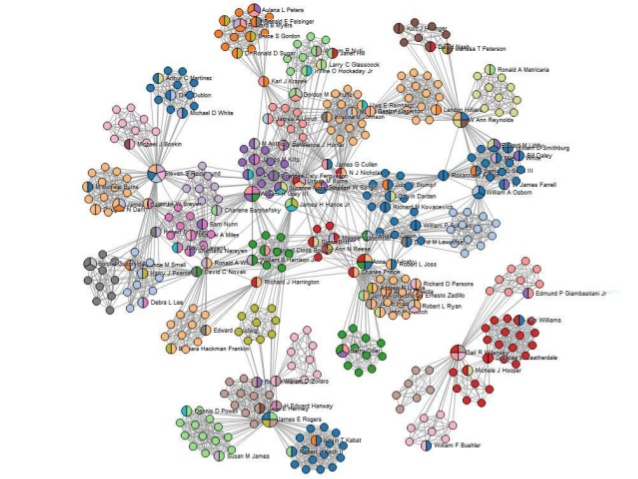
\includegraphics[width=1\textwidth]{images/9_social}
			\small 
			\caption{Cluster di amicizie in un social network } % \\ \textit{Fonte: SNAP Stanford}}
		\end{minipage}\hfill
		\pause
		\begin{minipage}[t]{.45\textwidth}
			\centering
			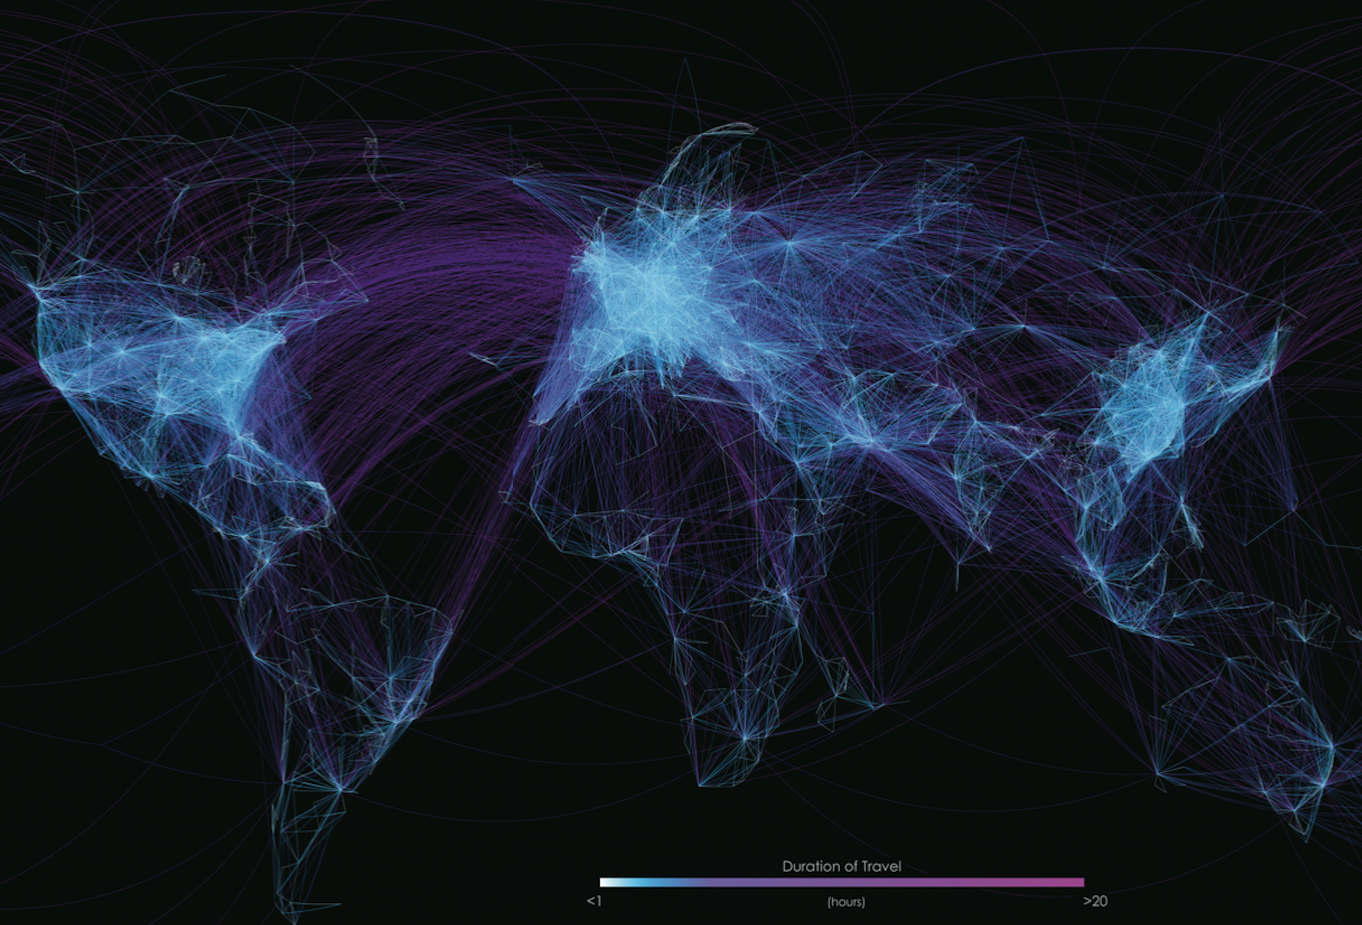
\includegraphics[width=1\textwidth]{images/7_flight}
			\small 
			\caption{Rotte dei voli commerciali} % \\ \textit{Fonte: Bio Diaspora, Toronto}}
		\end{minipage}
	\end{figure}
\end{frame}

\begin{frame}
	\frametitle{Indici di similarità}
	\centering
	
	\small
	\pause
	\begin{figure}[h]
		\begin{minipage}[t]{.48\textwidth}
			\centering
			\Large
			Jaccard
			\small
			\medskip
			\begin{equation*}
				J(A,B) = \frac{|A \cap B|}{|A \cup B|}
			\end{equation*}
			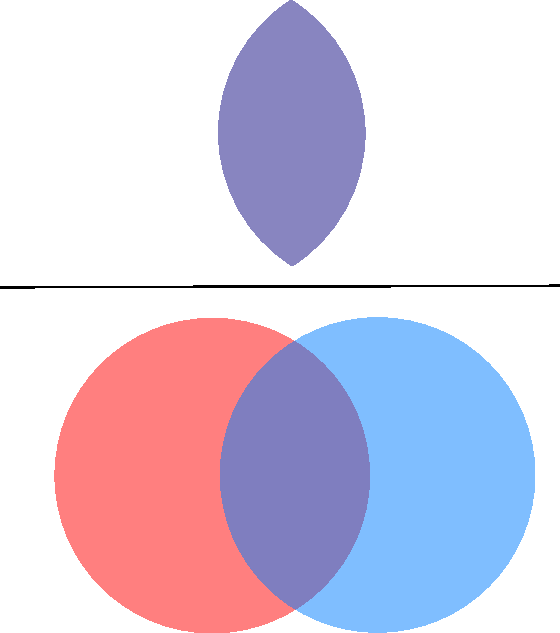
\includegraphics[width=0.5\textwidth]{images/4_jaccard}
		\end{minipage}\hfill
		\pause
		\begin{minipage}[t]{.48\textwidth}
			\centering
			\Large
			Bray-Curtis
			\small
			\medskip
			\begin{equation*}
			BC(A,B) = \frac{2 \times |A \cap B|}{|A| + |B|}
			\end{equation*}
			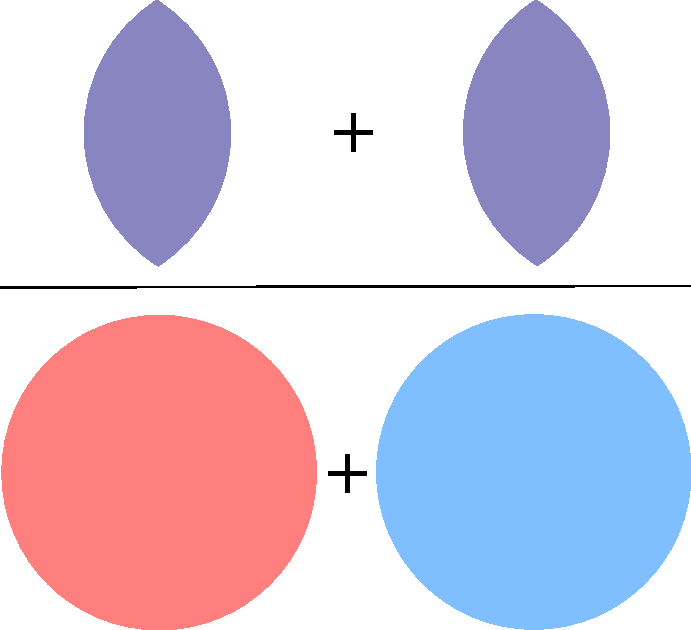
\includegraphics[width=0.6\textwidth]{images/5_bray_curtis}
			
		\end{minipage}\hfill		
	\end{figure}
	\small
	\pause
	
	$J(A,B) = BC(A,B) = 0$ se $A \cap B = \emptyset$\medskip
	
	$J(A,B) = BC(A,B) = 1$ se $A = B$ \phantom{$\cap \emptyset.$}
	
\end{frame}

\begin{frame}
	\frametitle{Reti etichettate e $q$-grammi}
	
	\textit{"Nessun uomo è un'isola, completo in se stesso; ogni uomo è un pezzo del continente, una parte del tutto."}
	\begin{flushright}
		\small \textit{John Donne}
	\end{flushright}
	
	\centering
	\textit{Analizzare non il solo nodo, ma anche la sua interfaccia verso l'esterno!}\\
	
	\pause
	
	Come modellare le interazioni?\\
	
	\pause
	
	\begin{figure}[h]
		\centering
		\begin{minipage}[t]{.49\textwidth}
			\centering
			Rete etichettata\medskip
			
			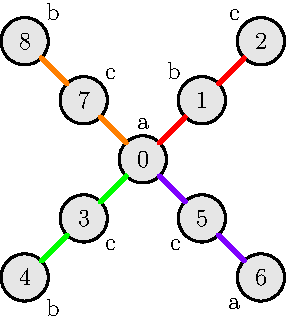
\includegraphics[width=0.5\textwidth]{images/11_labeled}
		\end{minipage}\hfill
		\pause
		\begin{minipage}[t]{.49\textwidth}
			
			\centering
			
			\textbf{q-grammi}: sottosequenza di $q$ elementi consecutivi in un testo
			
			+
			
			\textbf{q-path}: cammino di $q$ nodi \textit{distinti} collegati in un grafo \bigskip
			
			\small\pause
			
			\textbf{Esempio} $3$-grammi che terminano in $0$:
			\begin{itemize}
				\item $(2-1-0)$: \color{red}cba \color{black}
				\item $(4-3-0)$: \color{green}bca \color{black}
				\item $(6-5-0)$: \color{violet}aca \color{black}
				\item $(8-7-0)$: \color{orange}baa \color{black}
			\end{itemize}
		\end{minipage}
	\end{figure}

	
\end{frame}


\begin{frame}
	\frametitle{Frequenze dei $q$-grammi}
	
	\textbf{Notazione:}  
	\small \center	
	$f_X[w] = y \rightarrow$ Il $q$-gramma $w$ ha frequenza $y$ nei $q$-path che terminano in nodi di $X$\medskip
	
	\pause
	
	\textbf{Esempio:}  
	
	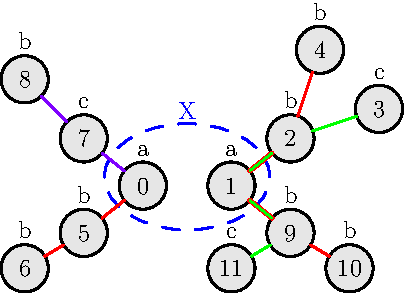
\includegraphics[width=0.4\textwidth]{images/12_freq}
		
	Dato $X = \{0, 1\}$ e $q=3$ abbiamo:
	\centering
	\begin{itemize}
		\item $f_X[bba] = 3$ (path: 4-2-1, 6-5-0, 10-9-1).
		\item $f_X[bca] = 1$ (path: 8-7-0).
		\item $f_X[cba] = 2$ (path: 3-2-1, 11-9-1).
	\end{itemize}
\end{frame}

\begin{frame}
	\frametitle{Il problema}
	
	\begin{flushleft}
		Dato un grafo $G=(V,E,L)$, etichettato su un alfabeto $\Sigma$, ed un intero $q$,
		calcolare la similarità tra due porzioni di grafo $A, B \subset V$ in base alle frequenze
		dei $q$-grammi dei $q$-path che terminano in nodi di $A$ e $B$.
	\end{flushleft}

	\pause
			
	Estendiamo i due indici ai $q$-grammi:

	\begin{equation*}\label{jaccard-sub}	
		J(A,B) = \frac{|A \cap B|}{|A \cup B|} \implies J(A,B) = \frac{ \Sigma_{w \in \Sigma^{q}} \min(f_{A}[w], f_{B}[w]) }{ \Sigma_{w \in \Sigma^{q}} f_{A \cup B}[w] }
	\end{equation*}

	\begin{equation*}\label{bray-sub}
		BC(A,B) = \frac{2 \times |A \cap B|}{|A| + |B|} \implies BC(A,B) = \frac{ 2 \times \Sigma_{w \in \Sigma^{q}} \min(f_{A}[w], f_{B}[w]) }{ \Sigma_{w \in \Sigma^{q}} (f_{A}[w] + f_{B}[w]) }
	\end{equation*}
	
\end{frame}

\begin{frame}
	\frametitle{Applicazioni pratiche}
	
	\pause
	\centering
	\begin{figure}[h]
		\centering
		\begin{minipage}[t]{.49\textwidth}
			\centering
			\textbf{NetInf}\medskip
			
			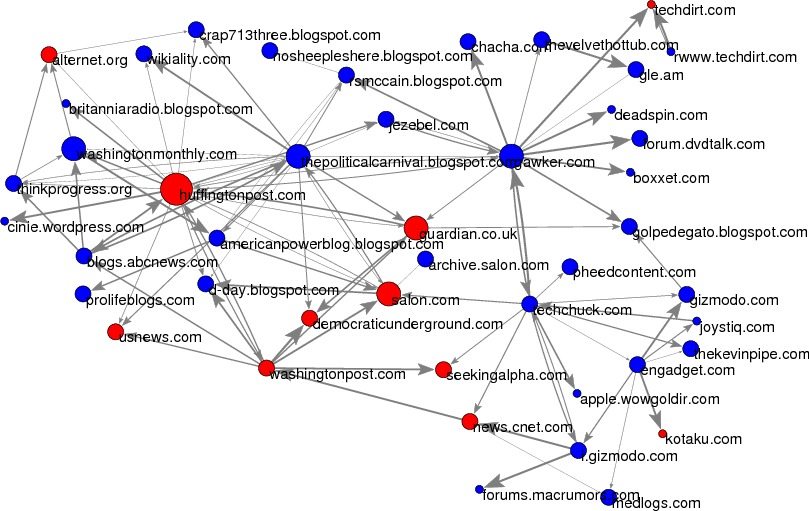
\includegraphics[width=0.9\textwidth]{images/4_netinf}
			\caption{Diffusione delle notizie tra i vari blog e siti di informazione statunitensi\\ \textit{Fonte: SNAP Stanford}}
		\end{minipage}\hfill
		\pause
		\begin{minipage}[t]{.49\textwidth}
			\centering
			\textbf{IMDb}\medskip
			
			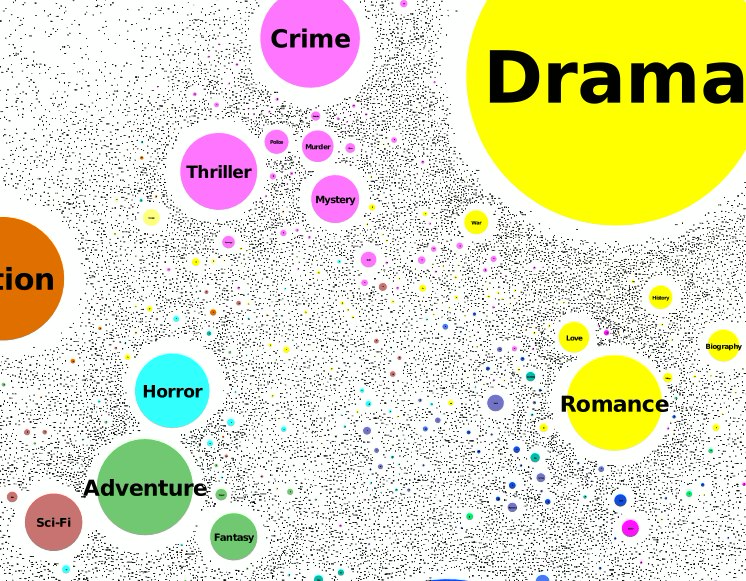
\includegraphics[width=0.9\textwidth]{images/6_imdb}
			\caption{Interazione tra i film con attori in comune\\ \textit{Fonte: IMDb}}
		\end{minipage}
	\end{figure}
\end{frame}
